% !TeX root = ../main.tex

\chapter{Coded Multi-Resource Systems with IDD}
\label{ch:coded}

This chapter introduces channel coding and iterative detection and decoding (IDD) into the multi-resource receiver. Motivated by the error-propagation problem observed in uncoded SIC receivers, the detector exchanges soft information with the FEC decoder and refines interference cancellation through iterations based on a priori information update. 
The block error rate (BLER) performance gap of MMSE-SIC-IDD, MMSE-PIC-IDD and MAP-IDD are clarified in coded multi-resource uplink NOMA system.
\begin{comment}
This chapter develops MMSE-SIC-IDD and compares it with MMSE-PIC-IDD and MAP-IDD to clarify the performance gap in coded multi-resource uplink NOMA system.
\end{comment}

\section{Introduction of IDD structure}
For coded systems, the detector is typically embedded in an iterative detection and decoding (IDD) receiver. In this structure, soft information is exchanged between the detector and the FEC decoder \cite{uchoa2015iterative,studer2011asic,li2024low}. The detector produces bit-level LLRs for the coded bits, while the decoder uses the code constraints to refine the reliability information and returns updated soft information to the detector, which is the a priori information of next detector calculation. 
In our simulations, the IDD receiver is implemented with a maximum number of iterations $t_{\max}$, and the final decoder output is used to make hard decisions on the transmitted bits. 

\begin{figure}
    \centering
    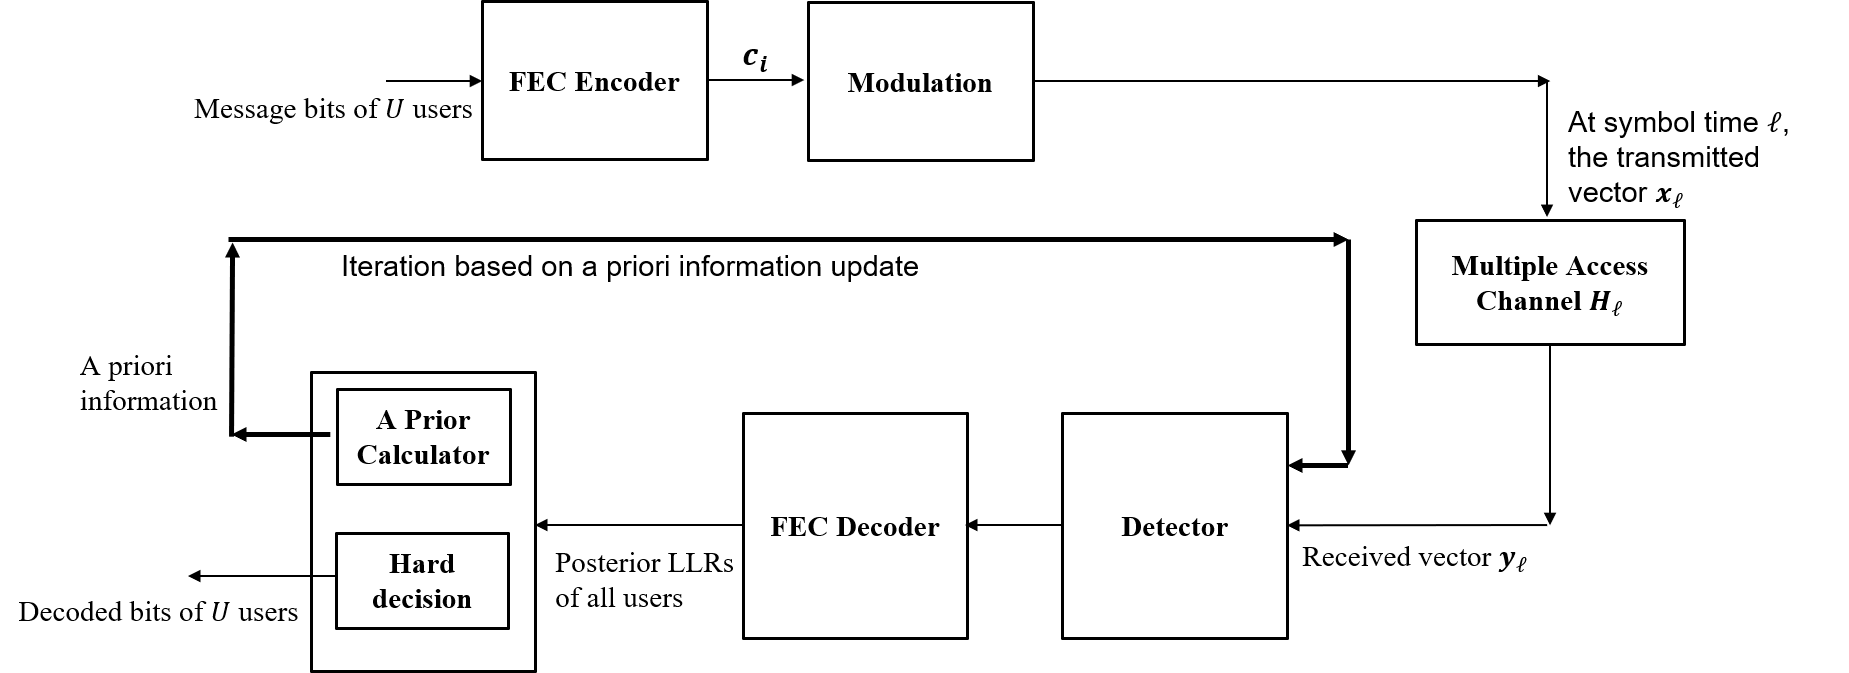
\includegraphics[width=0.9\linewidth]{figures/Chapter4/IDD_structure.png}
    \caption{Coded NOMA system with IDD receiver}
    \label{fig:IDD_structure}
\end{figure}

\section{Coded Multi-resource system model}
In this chapter, different users are allowed to employ different modulation schemes and different channel code lengths.
Let $\bm{c}_i$ denote user $i's$ transmitted codeword of length $N_{c,i}$
\begin{equation}
    \bm{c}_i=[c_{i,1},c_{i,2},\ldots,c_{i,N_{c,i}}]^T,
\end{equation}
After modulation, the codeword is grouped into $N_{s}$ modulation symbols. At symbol time $\ell$, the transmitted vector is
\begin{equation}
    \bm{x}_\ell=[x_{1,\ell},x_{2,\ell},\ldots,x_{U,\ell}]^T,
\end{equation}
Refer to equation \eqref{eq:multi resource model}, the received vector is
\begin{equation}
    \bm{y}_\ell=\bm{H}_\ell\bm{x}_\ell+\bm{n}_\ell.
    \label{eq:coded-symbol-model}
\end{equation}
In the block-fading simulations, $\bm{H}_1=\bm{H}_2=\cdots=\bm{H}_{N_s}$. For simplicity, we omit the subscript $\ell$, which denotes the process is dealing with $\bm{y_\ell}$. 
The overall block diagram of coded NOMA system with IDD receiver is shown in figure.~\ref{fig:IDD_structure}.

\section{MMSE-SIC-IDD}

In this section, we introduce the procedure of the MMSE-SIC-IDD receiver. The key feature of the structure is that interference cancellation in the SIC process is performed after channel decoding rather than immediately after detection.

\subsection{Receiver Procedure}
Following a similar procedure in section \ref{sec:MMSE SIC detection order}, the detection order can be obtained. For post-SINR ordering method, the additional $\bar{v}_i^{(t)}$ is considered and will be disscussed in section \ref{sec:Variance-Aware MMSE Filtering}. Assume the users are re-numbered from $1$ to $U$ according to this order. 

For user $i$, the detector first computes the bit-level LLRs $\bm{L}_{\bm{c}_i}$. The summation of these LLRs and a priori information are then passed to the FEC decoder of user $i$. After decoding, the decoder produces the a posteriori LLRs $\bm{L}^d_{\bm{c}_i}$, which are used to generate the decoded soft symbol estimate $\hat{\bm{s}}^d_i$. This decoded soft symbol estimate is then fed back to the MMSE-SIC detector for the next SIC stage, i.e., user $i+1$, where it is used to subtract the interference caused by user $i$. 
Intuitively, performing cancellation after decoding can improve the reliability of the cancelled signal and thus reduce error propagation in the SIC process.

Due to the successive decoding procedure, the extrinsic information of each user is collected asynchronously. Specifically, after decoding user $i$, the extrinsic LLRs are obtained as
\begin{equation}
    \label{eq:extrinsic LLR for next a priori update}
    \bm{L}^e_{\bm{c}_i} = \bm{L}^d_{\bm{c}_i} - \bm{L}^{in}_{\bm{c}_i},
\end{equation}
where $\bm{L}^{in}_{\bm{c}_i}$ is the input of decoder.
In this way, the decoded extrinsic information of all users is provided as a priori information to the MMSE-SIC detector in the following IDD iteration.

\subsection{Soft Information for a priori update}
\label{sec:Soft Information for a priori update}
Let $\mathcal{S}_i$ denote the modulation alphabet of user $i$, and let
$M_i=\log_2|\mathcal{S}_i|$ be the number of coded bits per modulation symbol. For a symbol
$s\in\mathcal{S}_i$, its binary label is written as
\begin{equation}
    \bm{b}_i(s)
    =
    [b_{i,0}(s),b_{i,1}(s),\ldots,b_{i,M_i-1}(s)] .
\end{equation}
Let $L^{(t)}_{c_{i},\ell,m}$ denote the a priori LLR of the $m$th coded bit in the $\ell$th modulation symbol of user $i$ at a priori update iteration $t$, with
\begin{equation}
    \label{eq:a priori LLR}
    L^{(t)}_{c_{i},\ell,m}
    =
    \log
    \frac{P^{a,(t)}(b_{i,\ell,m}=0)}
    {P^{a,(t)}(b_{i,\ell,m}=1)},
    \qquad
    L^{(0)}_{c_{i},\ell,m} = 0.
\end{equation}
The corresponding bit probability is
\begin{equation}
    P^{a,(t)}(b_{i,\ell,m}=b)
    =
    \frac{1}
    {1+\exp\left[-(1-2b)L^{(t)}_{c_{i},\ell,m}\right]},
    \qquad b\in\{0,1\}.
    \label{eq:bit-prior-from-llr}
\end{equation}
Assuming the interleaved coded bits are represented by independent bit priors at the demapper input, the a priori symbol probability is the product of its corresponding a priori bit probability\cite{tuchler2002minimum}, which is written as
\begin{equation}
    P^{a,(t)}_{i,\ell}(s)
    =
    \prod_{m=0}^{M_i-1}
    P^{a,(t)}(b_{i,\ell,m}=b_{i,m}(s)).
    \label{eq:symbol-prior-from-bit-priors}
\end{equation}
The soft symbol mean used for a priori update before detection is calculated according to the a priori symbol probability\cite{shapiro2005soft}, that is, 
\begin{equation}
    \mu^{(t)}_{i,\ell}
    =
    \mathbb{E}[x_{i,\ell}\mid \bm{L}^{(t)}_{c_{i},\ell}]
    =
    \frac{
    \sum\limits_{s\in\mathcal{S}_i}
    s P^{a,(t)}_{i,\ell}(s)}
    {\sum\limits_{s\in\mathcal{S}_i}
    P^{a,(t)}_{i,\ell}(s)} ,
    \label{eq:idd-general-soft-mean}
\end{equation}
and the corresponding symbol variance is
\begin{equation}
    \sigma^{2~(t)}_{i,\ell}
    =
    \frac{
    \sum\limits_{s\in\mathcal{S}_i}
    \abs{s}^2 P^{a,(t)}_{i,\ell}(s)}
    {\sum\limits_{s\in\mathcal{S}_i}
    P^{a,(t)}_{i,\ell}(s)}
    -
    \abs{\mu^{(t)}_{i,\ell}}^2 .
    \label{eq:idd-general-soft-var}
\end{equation}
For BPSK modulation with $0\mapsto +1$ and $1\mapsto -1$, equation \eqref{eq:idd-general-soft-mean} and \eqref{eq:idd-general-soft-var} reduce to
\begin{equation}
    \mu^{(t)}_{i,\ell}
    =
    \tanh\left(\frac{L^{(t)}_{c_{i},\ell,0}}{2}\right),
    \qquad
    \sigma^{2~(t)}_{i,\ell}
    =
    1-\abs{\mu^{(t)}_{i,\ell}}^2 .
\end{equation}
For simplicity, we consider the average variance of user $i$ over the coded block,that is,
\begin{equation}
    \label{eq:average variance of user i}
    \bar{v}^{(t)}_{i}
    =
    \frac{1}{N_s}\sum_{\ell=1}^{N_s}\sigma^{2~(t)}_{i,\ell},
\end{equation}
The variance matrix is defined as
\begin{comment}
To simplify the expression in the following equations, for the current a priori update $t$, we omit the update superscript in the variance matrix and rewrite it as
\end{comment}
\begin{equation}
    \bm{V}
    =
    \operatorname{diag}(\bar{v}_1^{(t)},\bar{v}_2^{(t)},\ldots,\bar{v}_U^{(t)}),
    \qquad
    \bar{v}_i^{(t)}>0.
    \label{eq:variance-matrix}
\end{equation}

When decoder feedback is reliable, $\bar{v}_i^{(t)}$ becomes small, indicating a higher probability of successful decoding for user \(i\) and consequently a smaller residual interference. 
Conversely, when decoder feedback is uncertain, he variance remains large, allowing the receiver to avoid overconfident cancellation.

\subsection{Variance-Aware MMSE Filtering}
\label{sec:Variance-Aware MMSE Filtering}
When all users' extrinsic information from the FEC decoder has been asynchronously collected, the variance-aware MMSE filter of user $k$ \cite[Eqs. (6), (7)]{studer2011asic} for next a priori based iteration can proceed with the coefficient
\begin{equation}
    \label{eq:variance-aware-mmse}
    \tilde{\bm{w}}^H_k
    =
    \bar{v}_k^{(t)}\bm{h}_k^H
    \left(
    \bm{H}\bm{V}\bm{H}^H + 2\sigma^2\bm{I}
    \right)^{-1}.
\end{equation}
the corresponding post-SINR can be written as 
\begin{equation}
    \label{eq:post-sinr-with-variance}
    \gamma^{\mathrm{post}}_k
    =
    \frac{\abs{\tilde{\bm{w}}^H_k\bm{h}_k}^2}
    {\sum_{j\ne k}\bar{v}_j^{(t)}\abs{\tilde{\bm{w}}^H_k\bm{h}_j}^2+2\sigma^2\norm{\tilde{\bm{w}}_k}^2}.
\end{equation}
Compared with equation \eqref{eq:coefficient} and \eqref{eq:post-sinr}, users with reliable a priori information contribute less uncertainty to the MMSE filtering process and SIC detection ordering.

\subsection{Decoder-Aided SIC Cancellation}

To simplify the expression in the following equations, we omit the subscript $\ell$, which denotes that the process is dealing with $\bm{y}_{\ell}$. The procedure goes back to MMSE-SIC stage 1, user 1 can benefit from the a priori information of users $2,\ldots,U$ by using
\begin{equation}
    \label{eq:idd-stage-one-residual}
    \bm{y}_{(1)}^{(t)}
    =
    \bm{y}
    -
    \sum_{j=2}^{U}
    \bm{h}_{j}\mu^{(t)}_{j}.
\end{equation}
At SIC stage $i>1$, the detection of user $i$ benefits from the FEC outputs of users $1,2,\ldots,i-1$ and from the a priori information of users $i+1,\ldots,U$. The residual vector for detecting user $i$ is constructed as
\begin{equation}
    \label{eq:idd-stage-i-residual}
    \bm{y}_{(i)}^{(t)}
    =
    \bm{y}
    -
    \sum_{j=1}^{i-1}
    \bm{h}_{j}\hat{s}^{d}_{j}
    -
    \sum_{j=i+1}^{U}
    \bm{h}_{j}\mu^{(t)}_{j}.
\end{equation}
The first summation cancels the users that have already been decoded in the current SIC pass by using the decoder-aided soft symbol estimates $\hat{s}^{d}_{j}$. This will be discussed in Section \ref{sec:LLR calculation and soft estimate}. The second summation cancels the users that have not yet been decoded in the current pass by using the a priori soft symbol mean $\mu^{(t)}_{j}$.
\begin{comment}
The cancellation term in equation \eqref{eq:idd-stage-i-residual} is different from that used in the uncoded MMSE-SIC detection in Chapter~\ref{ch:multi-resource}. In the uncoded case, the cancelled signal is obtained directly from the detector output at the current SIC stage, and this estimate is used for interference subtraction without explicitly modeling its remaining uncertainty in the next SIC stage.
In contrast, in the coded IDD receiver, users $1,\ldots,i-1$ have already passed through the FEC decoder in the current SIC pass. Therefore, it provides not only more reliable soft symbol estimates for cancellation, but also reliability information that can be used to characterize the remaining uncertainty after cancellation. Based on the reliable soft symbol estimates $\bm{h}_{j}\hat{s}^{d}_{j}$, the residual uncertainty of the cancellation is incorporated into the MMSE-SIC-IDD formulation through the cancellation residual variance $v_c^{\mathrm{can}}$. The detailed calculation of $v_c^{\mathrm{can}}$ is given in Section~\ref{sec:LLR calculation and soft estimate}.
\end{comment}
The cancellation term in equation \eqref{eq:idd-stage-i-residual} differs from that used in the uncoded MMSE-SIC detection. In the uncoded case, the cancelled signal is directly derived from the detector output at the current SIC stage, and the corresponding residual uncertainty is not explicitly considered in MMSE filtering. In the coded IDD receiver, however, users $1,\ldots,i-1$ have already been decoded in the current SIC pass and the outputs provide more reliable soft symbol estimates as well as reliability information for quantifying the remaining uncertainty after cancellation. Therefore, the decoder-aided cancellation is modeled together with its residual variance $\bar{v}_c^{can}$, whose detailed calculation is given in Section~\ref{sec:LLR calculation and soft estimate}.

Similar to the uncoded MMSE-SIC procedure in equation \eqref{eq:downsized channel matrix}, \eqref{eq:filter output stage i}, \eqref{eq:effective noise stage i} and \eqref{eq:mmse-sic-equivalent-scalar-channel}, the downsized channel matrix and the downsized variance matrix are used after each stage. The filter output for user $i$ is
\begin{equation}
    z^{(t)}_{i}
    =
    \tilde{\bm{w}}^H_i
    \bm{y}_{(i)}^{(t)},
\end{equation}
with equivalent scalar gain
\begin{equation}
    a^{(t)}_{i}
    =
    \tilde{\bm{w}}^H_i\bm{h}_i .
\end{equation}
The effective variance of the residual interference and noise with additional residual uncertainty is
\begin{equation}
    \sigma_{i,\mathrm{eff}}^{2~(t)}
    =
    \sum_{j>i}
    \bar{v}_j^{(t)}
    \abs{\tilde{\bm{w}}^H_i\bm{h}_j}^2
    +
    \sum_{c<i}
    \bar{v}_c^{can}
    \abs{\tilde{\bm{w}}^H_i\bm{h}_c}^2
    +
    2\sigma^2\norm{\tilde{\bm{w}}^H_i}^2 .
    \label{eq:idd-eff-var}
\end{equation}
\begin{comment}
The first term in \eqref{eq:idd-eff-var} comes from undecoded users whose interference is represented by the a priori variance $\bar{v}_j^{(t)}$. The second term is the cancellation residual $\bar{v}_c^{can}$, which is caused by the uncertainty of decoded users. The last term is the filtered noise variance. Therefore, 
\end{comment}
Unlike the uncoded MMSE-SIC detection, the coded receiver explicitly accounts for the residual uncertainty of decoder-aided cancellation.


\subsection{LLR calculation and soft estimate}
\label{sec:LLR calculation and soft estimate}
Define the set $\mathcal{S}_{i,m,b}$ is the subset of constellation symbols of user \(i\) whose $m^{th}$ bit label is equal to \(b\):
\begin{equation}
    \mathcal{S}_{i,m,b}
    =
    \{s\in\mathcal{S}_i:b_{i,m}(s)=b\},
    \qquad b\in\{0,1\}.
\end{equation}
After MMSE filtering and decoder-aided cancellation, the LLR of detector output is computed from $z_i^{(t)}$, the scalar gain $a_i^{(t)}$, the effective variance $\sigma_{i,\mathrm{eff}}^{2~(t)}$ and the a priori LLRs in equation \eqref{eq:a priori LLR}. 
The a priori symbol probability is given by equation \eqref{eq:symbol-prior-from-bit-priors}, where the bit probabilities are obtained from $L^{(t)}_{c_i,\ell,m}$ by the LLR-to-probability rule in equation \eqref{eq:bit-prior-from-llr}.
The subscript $\ell$ and superscript $(t)$ are omitted in the following scalar detection equations and LLR expressions respectively for compactness.
The detector produces an extrinsic bit-level LLR for the $m^{th}$ bit of user $i$, $L_{c_{i},m}$ \cite{tuchler2002minimum} by using the a priori information of the other bits in the same modulation symbol, but not the a priori information of the target bit itself:
\begin{equation}
    L_{c_{i},m}
    =
    \log
    \frac{
    \sum\limits_{s\in\mathcal{S}_{i,m,0}}
    \exp\left(
    -\frac{\abs{z^{(t)}_{i}-a^{(t)}_{i} s}^2}
    {\sigma_{i,\mathrm{eff}}^{2~(t)}}
    +
    \sum\limits_{\substack{m'=0\\m'\ne m}}^{M_i-1}
    \log P^{a,(t)}(b_{i,m'}=b_{i,m'}(s))
    \right)}
    {\sum\limits_{s\in\mathcal{S}_{i,m,1}}
    \exp\left(
    -\frac{\abs{z^{(t)}_{i}-a^{(t)}_{i} s}^2}
    {\sigma_{i,\mathrm{eff}}^{2~(t)}}
    +
    \sum\limits_{\substack{m'=0\\m'\ne m}}^{M_i-1}
    \log P^{a,(t)}(b_{i,m'}=b_{i,m'}(s))
    \right)} .
    \label{eq:idd-demapper-extrinsic-llr}
\end{equation}
\begin{comment}
    For BPSK modulation, equation \eqref{eq:idd-demapper-extrinsic-llr} reduces to the scalar LLR expression
    \begin{equation}
        L_{c_i}
        =
        \frac{4\abs{(a_i^{(t)})^*z_i^{(t)}}^2}
        {\sigma_{i,\mathrm{eff}}^{2~(t)}}.
        \label{eq:idd-bpsk-llr}
    \end{equation}
\end{comment}
The input of FEC decoder is the sum of the detector extrinsic bit LLR and the target-bit a priori LLR:
\begin{equation}
    L^{\mathrm{in}}_{c_i,m}
    =
    L_{c_{i,m}}
    +
    L_{c_i,m}.
    \label{eq:decoder-input-llr}
\end{equation}
The FEC decoder then produces posterior LLRs $\bm{L}^{d}_{\bm{c}_i}$ and will be used to form the decoder-aided soft symbol estimate for SIC cancellation. The calculation follows the same bit-probability, symbol-probability, and posterior-mean rules in equation \eqref{eq:bit-prior-from-llr}, \eqref{eq:symbol-prior-from-bit-priors}, and \eqref{eq:idd-general-soft-mean}, with the a priori LLRs is replaced by the decoder posterior LLRs. Therefore, for each symbol position $\ell$, the decoded soft estimate $\hat{s}^{d}_{i,\ell}$ is obtained from $\bm{L}^{d}_{\bm{c}_i}$ in the same way that $\mu^{(t)}_{i,\ell}$ is obtained from $\bm{L}^{(t)}_{c_i,\ell}$.

The only additional quantity required in the decoder-aided SIC process is the cancellation residual variance $\bar{v}_i^{\mathrm{can}}$, which is the second term of effective variance in equation \eqref{eq:idd-eff-var}. This quantity is computed according to $\hat{s}^{d}_{i,\ell}$ and follows the equation \eqref{eq:idd-general-soft-mean}--\eqref{eq:average variance of user i} with the soft symbol mean is replaced by the decoded soft estimate. 
\begin{comment}
This characterizes the remaining uncertainty after subtracting the decoder-aided soft estimate $\hat{s}^d_i$ from the received vector. When the decoder output is more reliable, the resulting $\bar{v}_i^{\mathrm{can}}$ becomes smaller, thereby reducing the residual interference contribution to the subsequent SIC stages.
\end{comment}

\paragraph{Summary of MMSE-SIC-IDD}
The overall procedure of the MMSE-SIC-IDD receiver is summarized in Algorithm~\ref{alg:mmse-sic-idd}. 

\begin{algorithm}[t]
\caption{MMSE-SIC-IDD receiver for one coded block}
\label{alg:mmse-sic-idd}
\begin{algorithmic}[1]
\STATE Initialize the a priori LLRs $L^{(0)}_{c_i,\ell,m}=0$ for all users, coded-symbol positions, and bit positions.
\FOR{$t=0,1,\ldots,t_{\max}$}
    \STATE Compute $\mu^{(t)}_{i,\ell}$ and $\sigma^{2~(t)}_{i,\ell}$ for all users.
    \STATE Form the variance matrix $\bm{V}$ from the block-averaged variances.
    \STATE Determine the detection order and re-number the users as $1,\ldots,U$.
    \FOR{$i=1,2,\ldots,U$}
        \STATE Compute the variance-aware MMSE filter in \eqref{eq:variance-aware-mmse}.
        \STATE Build $\bm{y}^{(t)}_{(i)}$ using \eqref{eq:idd-stage-one-residual} or \eqref{eq:idd-stage-i-residual}.
        \STATE Generate detector extrinsic LLRs using \eqref{eq:idd-demapper-extrinsic-llr}.
        \STATE Form the decoder input LLRs using \eqref{eq:decoder-input-llr}.
        \STATE Decode user $i$ and obtain $\hat{s}^{d}_{i}$ and $\bar{v}_i^{can}$.
    \ENDFOR
    \STATE Set the next a priori LLRs using \eqref{eq:extrinsic LLR for next a priori update}.
\ENDFOR
\STATE Make hard decisions from the final decoder outputs.
\end{algorithmic}
\end{algorithm}


\section{MMSE-PIC-IDD}
In this section, we introduce the MMSE-PIC-IDD receiver, which is a parallel interference cancellation (PIC) receiver that also exchanges soft information with the FEC decoder.
Compared to the successive interference cancellation (SIC), PIC cancels all other users in parallel instead of successively decoding one user at a time \cite{studer2011asic}. For user $k$, the residual vector is calculated by substracting all other users:
\begin{equation}
    \bm{y}^{(t)}_{k,\ell}
    =
    \bm{y}_\ell
    -
    \sum_{j\ne k}\bm{h}_j\mu^{(t)}_{j,\ell}.
    \label{eq:pic-residual}
\end{equation}
The variance-aware MMSE filter follows the same form as equation \eqref{eq:variance-aware-mmse}, and the LLR calculation follows the MMSE-SIC procedure. 

PIC avoids SIC ordering and reduces decoding latency because users can be processed in parallel. However, it relies directly on the a priori information of all interfering users, so the iteration of a priori information update is especially important. SIC, in contrast, performs ordered stage-by-stage cancellation and can additionally use decoded-user feedback from earlier stages in the same pass, albeit at the expense of ordering dependence and increased latency.
\begin{comment}
This difference makes PIC and SIC complementary references: PIC represents a more parallel receiver whose cancellation quality is dominated by a priori reliability, whereas SIC represents a sequential receiver that can exploit current decoder outputs at the cost of ordering dependence and longer latency.
\end{comment}




\section{MAP-IDD}

In this receiver, the detector follows the maximum a posteriori (MAP) rule. The detector-decoder exchange follows the same IDD structure described previously. The detector produces bit-level LLRs, the FEC decoder refines them, and the decoder extrinsic information is fed back to the detector as the a priori information for the next update.

In this section, we mainly focus on how the a priori information is operated in the MAP detector. Similar to Section~\ref{sec:Detection principle for GDMA}, the MAP detector considers all possible superimposed signals. For simplicity, the subscript $\ell$ is omitted in this section, which means that the receiver is processing the $\ell$th transmission symbol. The possible superimposed signal set is written as
\begin{equation}
    \mathcal{S}
    =
    \left\{
    \bm{s}_{0},
    \bm{s}_{1},
    \ldots,
    \bm{s}_{N_L-1}
    \right\},
\end{equation}
where
\begin{equation}
    N_L
    =
    \prod_{k=1}^{U}|\mathcal{S}_k|
    =
    2^{\sum_{k=1}^{U}M_k}.
\end{equation}
The $l^{th}$ possible superimposed signal is generated by one combination of all users' modulation symbols. Let this combination be
\begin{equation}
    \bm{x}_{l}
    =
    [x_{1,l},x_{2,l},\ldots,x_{U,l}]^T,
    \qquad
    x_{k,l}\in\mathcal{S}_k .
\end{equation}
Then the corresponding superimposed signal is
\begin{equation}
    \bm{s}_{l}
    =
    \bm{H}\bm{x}_{l}.
\end{equation}

For example, consider three users employing BPSK, QPSK, and 16QAM, respectively. In this case,
\[
    |\mathcal{S}_1|=2,\qquad
    |\mathcal{S}_2|=4,\qquad
    |\mathcal{S}_3|=16,
\]
and the MAP detector needs to consider
\[
    N_L=2\times 4\times 16=128
\]
possible superimposed signals for each received symbol. One possible combination is, for example:
\begin{equation}
    \bm{x}_{l}
    =
    \left[
    x_{1,l},
    x_{2,l},
    x_{3,l}
    \right]^T
    =
    \left[
    +1,
    \frac{1+j}{\sqrt{2}},
    \frac{1+3j}{\sqrt{10}}
    \right]^T ,
\end{equation}
where the first entry is selected from the BPSK constellation, the second entry is selected from the QPSK constellation, and the third entry is selected from the 16QAM constellation. This symbol combination produces one possible superimposed signal
\begin{equation}
    \bm{s}_{l}
    =
    \bm{H}
    \left[
    +1,
    \frac{1+j}{\sqrt{2}},
    \frac{1+3j}{\sqrt{10}}
    \right]^T .
\end{equation}
The MAP detector repeats this construction for all possible symbol combinations.

Without a priori information, all possible superimposed signals are assumed to be equally likely. In MAP-IDD, however, the detector uses the a priori LLRs from the previous IDD update to weight each possible superimposed signal. From equation \eqref{eq:bit-prior-from-llr}, the a priori probability of the $l$th possible superimposed signal is
\begin{equation}
    P^{a,(t)}_{l}
    =
    \prod_{k=1}^{U}
    \prod_{m=0}^{M_k-1}
    P^{a,(t)}
    \left(
    b_{k,m}
    =
    b_{k,m}(x_{k,l})
    \right).
    \label{eq:map-idd-prior-superimposed}
\end{equation}
Therefore, the APP of the $l$th possible superimposed signal is proportional to
\begin{equation}
    P^{(t)}(\bm{s}_{l}|\bm{y})
    \propto
    \exp\left(
    -\frac{
    \left\|
    \bm{y}
    -
    \bm{s}_{l}
    \right\|^2}
    {2\sigma^2}
    \right)
    P^{a,(t)}_{l}.
    \label{eq:map-idd-app-superimposed}
\end{equation}
Equation~\eqref{eq:map-idd-app-superimposed} shows that the a priori information changes the probability of each possible superimposed signal according to its bit labels. 
\begin{comment}
If the bit labels of a possible superimposed signal are more consistent with the decoder feedback, then its a priori probability becomes larger and the MAP detector gives it a larger APP weight.
\end{comment}

For the $m^{th}$ bit of user $k$, the detector output LLR is obtained by summing the APPs of all possible superimposed signals whose corresponding bit is equal to $0$ or $1$:
\begin{equation}
    L^{\mathrm{MAP}}_{c_k,m}
    =
    \log
    \frac{
    \sum\limits_{l:b_{k,m}(x_{k,l})=0}
    P^{(t)}(\bm{s}_{l}|\bm{y})
    }
    {
    \sum\limits_{l:b_{k,m}(x_{k,l})=1}
    P^{(t)}(\bm{s}_{l}|\bm{y})
    } .
    \label{eq:map-idd-llr}
\end{equation}
After the detector LLRs are derived synchronously for all users, the subsequent IDD procedure follows the same steps described previously.

MAP-IDD provides a strong coded joint-detection ability because it evaluates the APPs over all possible superimposed signals. However, its complexity increases with $N_L=\prod_{k=1}^{U}|\mathcal{S}_k|$, and therefore grows rapidly as the number of users or modulation order increases.

\section{Coded Simulation Results}
For the MMSE-SIC-IDD receiver, post-SINR ordering is used. In the four-user case and overloaded scenarios with more than four users, dynamic post-SINR ordering is considered. In this ordering strategy, the detection order is updated after each SIC stage. Accordingly, the post-detection SINR in equation \eqref{eq:post-sinr-with-variance} is recalculated at every SIC stage based on the remaining undecoded users.

We compare block error rate (BLER) of three different receiver structures that mentioned above. The simulations employ a $(1008,504)$ LDPC code over a independent block-fading channel for every user of each resource. The number of a priori information update iterations is denoted by $t_{max}$, where $t_{max}=0$ means no a priori information update is used. 2-resources is used in our system and BPSK modulation for each user unless otherwise specified. 
$\bar{E}_b$ in the simulations represent the average transmit energy per bit per user, normalized by the number of resources.

The objective of these simulation results is to investigate the effects of decoder feedback, SIC/PIC-based interference cancellation, system loading, and modulation order on the performance of coded multi-user receivers.

%\begin{comment}
\begin{figure}[htbp]
    \centering
    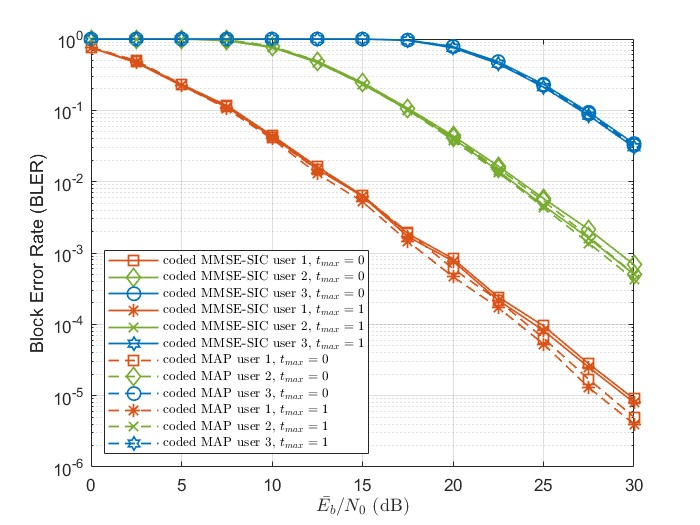
\includegraphics[width=0.9\linewidth]{figures/Chapter4/multi_resource_beta0.1_MMSESIC_BLER.jpg}
    \caption{BLER of MMSE-SIC-IDD and MAP-IDD with $R=2$, $(\beta_1,\beta_2,\beta_3)=(1,0.1,0.01)$, $t_{\max}=0$ and $t_{\max}=1$.}
    \label{fig:multi_resource_beta0.1_MMSESIC_BLER}
\end{figure}
\begin{figure}[htbp]
    \centering
    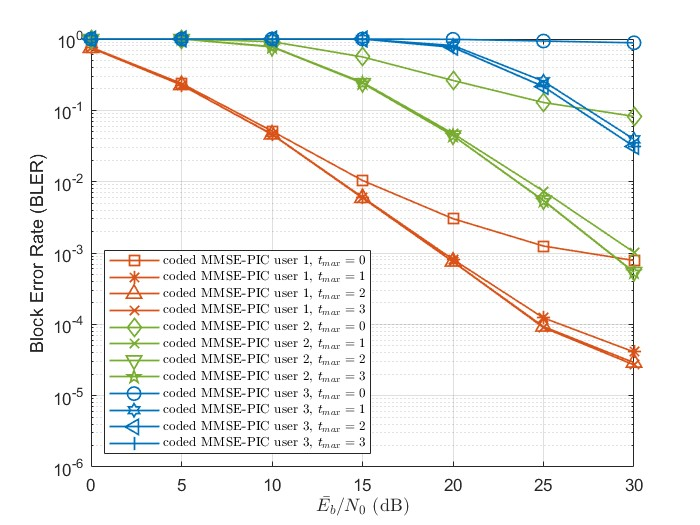
\includegraphics[width=0.9\linewidth]{figures/Chapter4/multi_resource_beta0.1_MMSEPIC_BLER.jpg}
    \caption{BLER of MMSE-PIC-IDD with $R=2$, $(\beta_1,\beta_2,\beta_3)=(1,0.1,0.01)$, $t_{\max}=0,1,2,3$}
    \label{fig:multi_resource_beta0.1_MMSEPIC_BLER}
\end{figure}
%\end{comment}

Figure.~\ref{fig:multi_resource_beta0.1_MMSESIC_BLER} shows the BLER performance of MMSE-SIC-IDD and MAP-IDD with unequal-$\beta_k$ case. 
Figure.~\ref{fig:multi_resource_beta0.1_MMSEPIC_BLER} shows the BLER performance of MMSE-PIC-IDD with unequal-$\beta_k$ case.
It's observed that MMSE-PIC-IDD strongly relies on reliable a priori information update because parallel cancellation relies directly on the a priori-based soft means of all interfering users. Compare with MMSE-SIC-IDD and MAP-IDD in figure.~\ref{fig:multi_resource_beta0.1_MMSESIC_BLER}, the performance is closed to all users, indicating that decoder-aided soft cancellation effectively reduces residual interference.

%\begin{comment}
\begin{figure}[htbp]
    \centering
    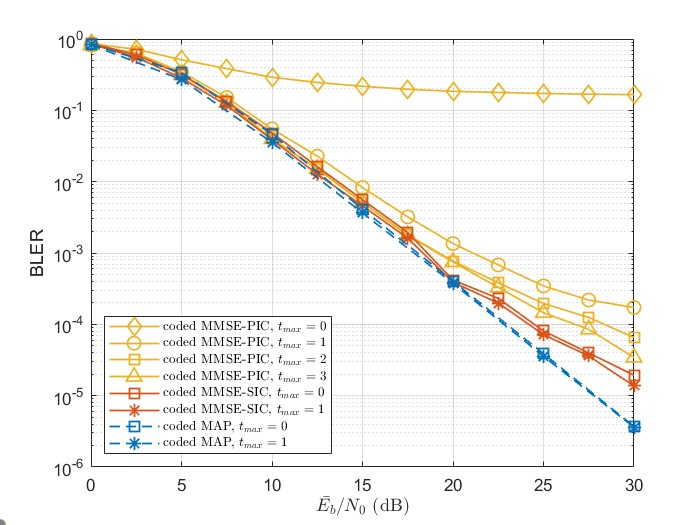
\includegraphics[width=0.9\linewidth]{figures/Chapter4/multi_resource_beta1_U3_BLER.jpg}
    \caption{BLER of different receiver structures with $R=2$, $U=3$ and $(\beta_1,\beta_2,\beta_3)=(1,1,1)$.}
    \label{fig:multi_resource_beta1_U3_BLER}
\end{figure}
%\end{comment}

Figure.~\ref{fig:multi_resource_beta1_U3_BLER} shows the BLER performance of MMSE-PIC-IDD, MMSE-SIC-IDD and MAP-IDD with equal-$\beta_k$ case.
For the MMSE-PIC-IDD scheme, convergence of the BLER is nearly achieved by $t_{\max}=3$. Consequently, the remaining simulations in this chapter are conducted solely using $t_{\max}=3$.
Compared with the MMSE-SIC-IDD and MAP-IDD, the performance is also closed, while MAP-IDD is slightly better in the high-SNR region.
It can also be observed that for both unequal-$\beta_k$ case and equal-$\beta_k$ case, the gain from increasing the value of $t$ is limited. This is due to the assumption of a block fading channel and the relatively moderate system loading.

%\begin{comment}
\begin{figure}[htbp]
    \centering
    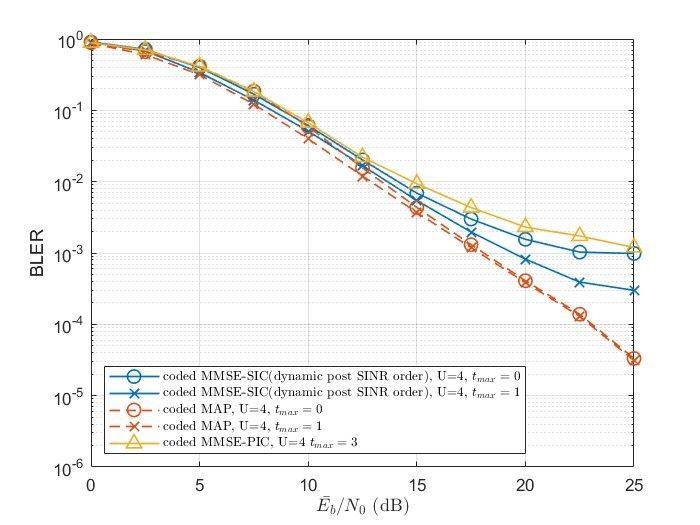
\includegraphics[width=0.9\linewidth]{figures/Chapter4/multi_resource_beta1_U4_BLER.jpg}
    \caption{BLER of different receiver structures with $R=2$, $U=4$ and $\beta_k=1$.}
    \label{fig:multi_resource_beta1_U4_BLER}
\end{figure}

\begin{figure}[htbp]
    \centering
    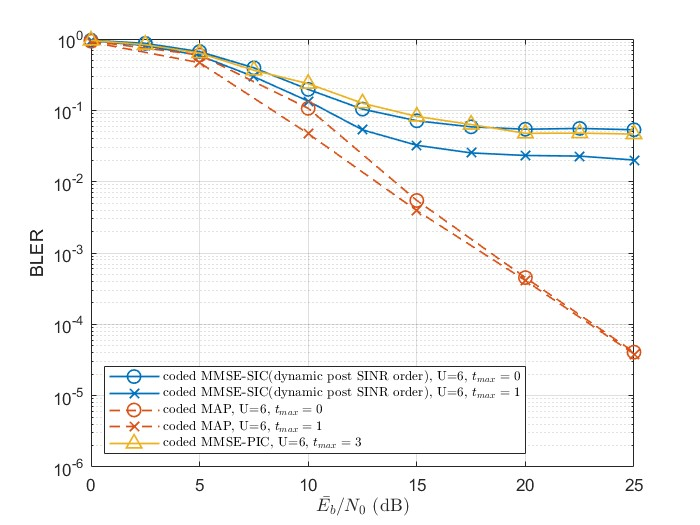
\includegraphics[width=0.9\linewidth]{figures/Chapter4/multi_resource_beta1_U6_BLER.jpg}
    \caption{BLER of different receiver structures with $R=2$, $U=6$ and $\beta_k=1$.}
    \label{fig:multi_resource_beta1_U6_BLER}
\end{figure}
%\end{comment}

Figure.~\ref{fig:multi_resource_beta1_U4_BLER} and ~\ref{fig:multi_resource_beta1_U6_BLER} are the case of 4-user and 6-user respectively. It can be seen that MAP-IDD maintains superior BLER performance owing to its near-optimal detection capability, whereas MMSE-based receivers becomes more sensitive to the increase in the number of user.




%\begin{comment}
\begin{figure}[htbp]
    \centering
    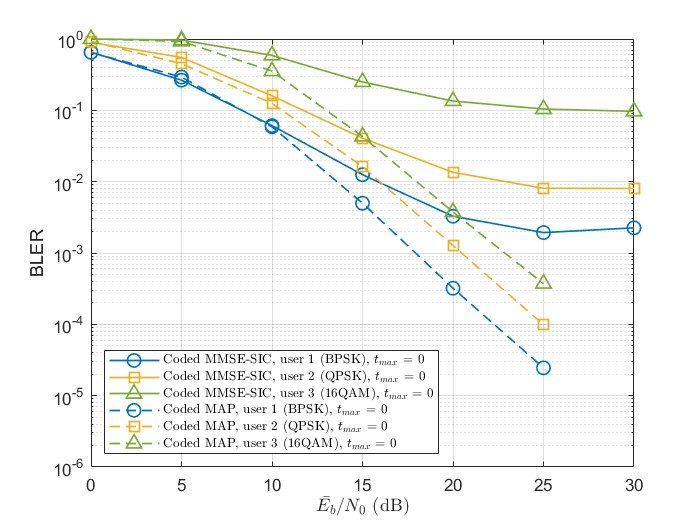
\includegraphics[width=0.9\linewidth]{figures/Chapter4/U3_BPSK_QPSK_16QAM_beta1_ite0.jpg}
    \caption{BLER of MMSE-SIC-IDD and MAP-IDD with $R=2$, $U=3$ and $\beta_k=1$. (BPSK, QPSK, 16QAM) is used. $t_{\max}=0$}
    \label{fig:U3_BPSK_QPSK_16QAM_beta1_ite0}
\end{figure}


\begin{figure}[htbp]
    \centering
    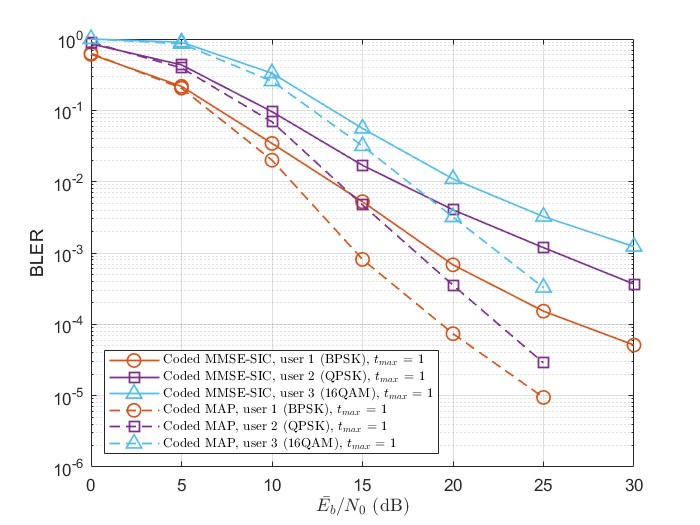
\includegraphics[width=0.9\linewidth]{figures/Chapter4/U3_BPSK_QPSK_16QAM_beta1_ite1.jpg}
    \caption{BLER of MMSE-SIC-IDD and MAP-IDD with $R=2$, $U=3$ and $\beta_k=1$. (BPSK, QPSK, 16QAM) is used. $t_{\max}=1$}
    \label{fig:U3_BPSK_QPSK_16QAM_beta1_ite1}
\end{figure}
%\end{comment}

Figure.~\ref{fig:U3_BPSK_QPSK_16QAM_beta1_ite0} and ~\ref{fig:U3_BPSK_QPSK_16QAM_beta1_ite1} consider three users using modulation (BPSK, QPSK, 16QAM). This two figures represent $t_{max}=0$ and $t_{max}=1$, respectively. 
Compare with BPSK modulation for every user, MAP-IDD can benefit from a priori information update even under block fading channel, since decoder feedback helps refine the APP weights of possible superimposed signals.


\section{Comparison and summary}

The simulation results show that the IDD is effective for coded multi-resource NOMA receivers, but the amount of gain depends on the detector type, system loading, and modulation order. For MAP-IDD, the detector already provides highly reliable soft information. Therefore, the additional gain from the a priori information update is smaller than that of the MMSE-based receivers in simple BPSK cases. However, MAP-IDD still achieves the best BLER performance in all simulated scenarios and remains robust when the number of users or modulation order~increases.

MMSE-SIC-IDD provides a favorable tradeoff between performance and complexity. By combining dynamic post-SINR ordering, variance-aware MMSE filtering, and decoder-aided cancellation, it can approach MAP-IDD in the three-user case and still performs well in the four-user case while BPSK modulation is used for every user. However, it is still based on linear filtering and sequential cancellation. When the system becomes heavily loaded, the  residual interference causes a clear performance floor.

MMSE-PIC-IDD has the advantage of parallel processing and lower receiver latency because all users can be detected simultaneously. However, its cancellation quality strongly depends on the reliability of the a priori information.

